\chapter{Preliminaries}
\label{chp:preliminaries}

Motion planning is the task of manipulating a robot's configurations so that,
given an initial and goal state or posture, the planner, is able to create a
sequence of actions that gives a feasible or optimal path through the
overarching planning environment, usually referred to as the world space. Thus a
motion planner can be seen as a machine which given an input: a world, and
initial and goal states, produces a sequence of actions to move the robot from
its initial to the desired goal configuration. This plan is then passed on to
the trajectory generator in the system. Generally, planners can be separated
into complete and non-complete planners, where being a complete planner means
that given enough time, all motion planning problems are solvable, only the
solution is NP-Hard~\cite{Lav06}, a non-complete planner makes no such
guarantess. Thus feasible solutions will have to make a compromise. A lot of
planners in use today are probabilistically complete, meaning that they converge
to a optimal solution given infinite time. There is a difference between on-line
and off-line motion planning, whereas the offline algorithm plans in a static
environment, the online algorithm is run continuously. However an on-line
algorithm can be simulated by running an offline algorithm repeatedly for short
intervals of time. However, this comes with the drawback, that no guarantee can
be made for completing the task at hand \cite{Lav06}.

\section{The mathematical framework}

In order to build, model and reason about a motion planning problem, certain
nomenclature and defininitions need to be standardized. A mathematical model of
the world, and the robot and its dynamics is necessary for clearly and precisely
reasoning about the problem at hand. Therefore the following sections creates
the mathematical definitions which is needed to create understand and interpret
the following chapters. For the dedicated reader, a more in depth introduction
can be found in \cref{sec:first-app}.

\subsection{The Robot and World Model}

First of all the robot and the overarching motion planner needs a world in which
a plan is to be created and executed. In this thesis the world space is a
2-dimensional plane, and is defined as:
\[
  \modelworld = \R^2
\]
In a real world planning problem not all parts of the \modelworld{} is
traversable by the robot. As an example, in a forest, treetrunks, branches, and
other inhabitants of the forest vegetation will be intraversable for a robot,
and hence these obstacles needs to be modelled. As obstacles inhabit the world
space, they will be modelled as subsets of the \modelworld, the same goes for
the robot body.
\[
  \modelrobot,\, \modelobstacle \subset \modelworld
\]

Next the robot needs to be able to move around in the world space. This is done
through a rigid body transformation on the robot model
\[
  h : \modelrobot\ \rightarrow \modelworld
\]


\subsubsection{Configuration Space}

However, the robot is more than a set of points in the world space. For example
a simple model of a car needs to know its heading as well. This information will
be referred to as the configuration space of the robot
(\modelconfigurationspace). For a simple car model this can be encoded in a
simple three dimensional vector holding the \(x\), \(y\), and \(\theta\)
parameters, like so
\[
  \modelconfigurationspace \subset SE(2),
\]
which encompass all the states the robot can be in during planning. \(SE(2)\)
stands for \textit{Special Euclidean two}, and is defined as \(SE(2) = \R^2
\times \mathcal{S}\).

As the robot lives in the world space, a subset of a robot's configuration can
be in collision with an obstacle.
\[
  \modelconfigurationspaceobst{} = \set{q \in \modelconfigurationspace{} \mid
    \mathcal{A}(q) \cap \modelobstacle{} \neq \emptyset}
\]
In the same way the free configuration space is defined as
\[
  \modelconfigurationspacefree{} = \mathcal{U} \setminus
  \modelconfigurationspaceobst{}
\]

More generally, the configuration space is a model for a wide variety of motion
planning problems. It is a manifold that arise from the transformations applied
to the robot. Thus in order to solve a motion planning problem, a search must be
performed in the configuration space. Thus the motion planning problem is now
made into a question of finding the best path to traverse the given
manifold~\cite{Lav06}.

\subsection{Action Space}

With the configuration space, and robot motion in the world space defined, the
next problem is to control the movement of the robot model, which is where the
\textit{action space} comes in. The action space is the set of inputs that can
be applied at any given state the robot is in. Thus one can model the action
space as a function of the robot's state.
\[
  \modelactionspace(\x) = \set{\uin \in \modelactionspace \mid \modelactionspace(\x)
    \neq \emptyset }
\]

\subsection{Initial and Goal States}

A planning problem needs to have an initial condition, and a goal state or a set
of states in the configuration space. Both the initial, and goal states can be
sets of states, meaning that it is not necessary to arrive specifically at the
target point. Mathematically the initial and goal sets is defined as
\begin{align*}
  \mathcal{X}_0 &= \set{ \x \in \modelconfigurationspace{} \mid g_i(\x) \leq a_i,
                  \, \forall i = 1,\ldots N_j} \\
  \mathcal{X}_{end} &= \set{ \x \in \modelconfigurationspace{} \mid g_i(\x) \leq
                      a_i, \, \forall i = 1,\ldots N_k}
\end{align*}
which defines the initial and final states as subsets of the
\modelconfigurationspace{} bounded by inequality constraints, such that the
intial and goal states are semi-algebraic sets.

\subsection{Dynamics}

The model of the robot has so far been unconstrained and free to move in all
directions as it please under an affine transformation. This representation does
not encompass the dynamics a system might have, which constrains the direction
and speed in which a model can move. In the case of a first order model (\ie it
does not take accelerations into account) the constraints are represented as a
differential equation of the form:
\[
  \dot{\x} = f(\x,\uin)
\]
and can optionally be extended to entail uncertainty
\[
  \dot{\x} = f(\x,\uin,\w)
\]
where \(\x\) is the configuration, \(\uin\) is the system input control, and
\(\w\) is an uncertainty term.

\subsubsection{Discrete motion planning}

Mentioned in the introduction, motion planning problems are in general NP-hard.
One way of making the problem more tractable is to discretize the problem. The
discrete motion planning problem employs all the same definitions as the
continuous case for the world and robot model, only all points are discrete in
time \(t_k\) for some \(k\). Therefore, let \(\mathcal{X}\) be the discrete
state space, and \(\mathcal{U}(x_k)\) be the set of actions available at each
point \(\x_k \in \mathcal{X}\). Then the state transition equation is now
written as:
\[
  \x_{k+1} = f(\x_k, \uin_k)
\]

\subsubsection{Representation of the plan}

The plan that the motion planner makes for a robot in the configuration space is
represented as a trajectory. A trajectory is a path with an additional time
parameter, so that the path through configuration space is now time variant.
This is represented as a function \(\phi(\alpha) \colon [0,1] \rightarrow
\mathcal{X}\), where \(\mathcal{X}\) is the configuration space of the vehicle,
with the time parameter added the trajectory is represented as a
time-parameterized function of the kind \(\pi(t) \colon [0,T] \rightarrow
\mathcal{X}\), where \(T\) is the planning horizon (\ie the endtime).

\subsection{Planning Under Uncertainty (Decision Theoretic Planning)}

All real life motion planning problems are faced with some level of uncertainty,
as errors can arise from a multiple of sources, whereas the most prevalent ones
are uncertainty in motion, sensing, or the environment.

Thus the exact system state is never exactly known. Therefore planning under
uncertainty is done in what~\cite[LaValle]{Lav06} refers to as the belief space,
which is a description of the state space using probability distributions. The
belief space is a general structure for working with plans under conditions of
uncertainty. Thus planning can be done mostly as it is done in a normal state
space, albeit in a higher dimension. Thus the state transition function can be
written as
\[
  \phi_{k+1} = f_{\mathcal{I}}\left( \phi_k, \mu_k, y_{k+1} \right)
\]

If the discrete state space model is expanded to include \(\w\) as the space of
uncertain actions, and \(\w_k\) is the action applied by an uncertain source at
time step \(k\), then the state transition transition is modeled as
\[
  \x_{k+1} = f(\x_k,\uin_k,\theta_k)
\]
As the uncertain actions are not available beforehand, that is -- \(\w_ k\) is
not given, the model turns into
\[
  X_{k+1} = \set{ \x_{k+1} \in X \mid \exists\theta_k \in \Theta(\x_k,\uin_k)
    \text{ such that } \x_{k+1} = f(\x_k,\uin_k,\theta_k)}
\] \cite{Lav06}.

\subsection{Reachable sets}
\label{subsec:reachable-set}

Of particular interest to the \rrtfunnel{} algorithm is the reachable set. A
reachable set is all the configurations that the robot can be in if started from
a particular point in the configuration space. Had there been no constraints on
the movement of the robot the reachable set would simply be the entirety of the
configuration space. However, the simple car model has both \textit{kinodynamic}
and \textit{non-holonomic} constraints. This leads to the car not necessarily
being able to reach all the states in the state-space from a given starting
point -- at least not given a timeframe. This idea is important as it leads to
the funnel definitions that makes up the backbone of this thesis. As an example,
the reachable set for the \textit{Dubins car} (which is a simple car model, with
a constant velocity, and a control on the heading of the vehicle) is visualized
in~\cref{fig:reachable-set-dubin}.

\begin{figure}
  \centering \documentclass[border=3mm,tikz]{standalone}
\begin{document}
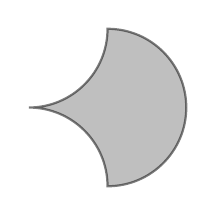
\begin{tikzpicture}
  \draw [black, fill=gray, opacity=.5, thick] (0,0) arc (270:360:1cm) -- (1,1) arc (90:-90:1cm)  -- (1,-1) arc (0:90:1cm);
\end{tikzpicture}
\end{document}
  \caption{The reachable set for a dubins car model after some time \(T\).}
  \label{fig:reachable-set-dubin}
\end{figure}

\subsection{Motion primitives}

The backbone of the \rrtfunnel{} algorithm is the composition of robust motion
primitives in order to construct a path to the target configuration. A motion
primitive is a constant action applied over fixed time intervals. It is one or
more actions collected into one discrete action. As an example, the action the
\textit{Dubin's car} employs is steering the angle of the wheels. Setting the
angle to a constant over a time interval can be a motion primitive, however, it
is more easily thought of as a collection of actions over time, which embodies
one bigger, more abstract action. For the car this could be \textit{go
  straight}, \textit{turn left}, etc. In this way, a collection of actions can
be thought of as one simple action. The robustness signifies that it is robust
in the face of uncertainty, meaning that if the uncertainty encountered is
within the bounds of the model, the motion primitives will be able accomplish
their task even in the face of this disturbance.

\section{Funnels}

A \textit{Funnel} is a parametrization of the reachable set of a dynamical
system. This means that a \textit{Funnel} holds all the states the dynamical
system can be in during a planning task. Mathematically the reachable set of the
system is defined as
\[
  \bar{\x}(0) \in \mathcal{X}_0 \implies \bar{\x}(t) \in F(t), \forall t \in
  \sqb{0,T}
\]
where \(\mathcal{X}_0\) is the set of initial conditions, \(\sqb{0,T}\) the time
interval, and \(F(t)\) is the set of states that the system can be in at time
\(t\). Although this thesis concerns itself with approximating the reachable set
through \textit{Lyapunov} functions, a useful analogy is imagining the funnel
created through \textit{Monte-Carlo} simulation, where the \textit{Funnel} would
be the set of all the paths traversed by the dynamical system at hand. For a
simple car model, monte-carlo simulation of nine starting points along the
y-axis looks like~\cref{fig:monte-carlo-sim}.

\begin{figure}
  \centering 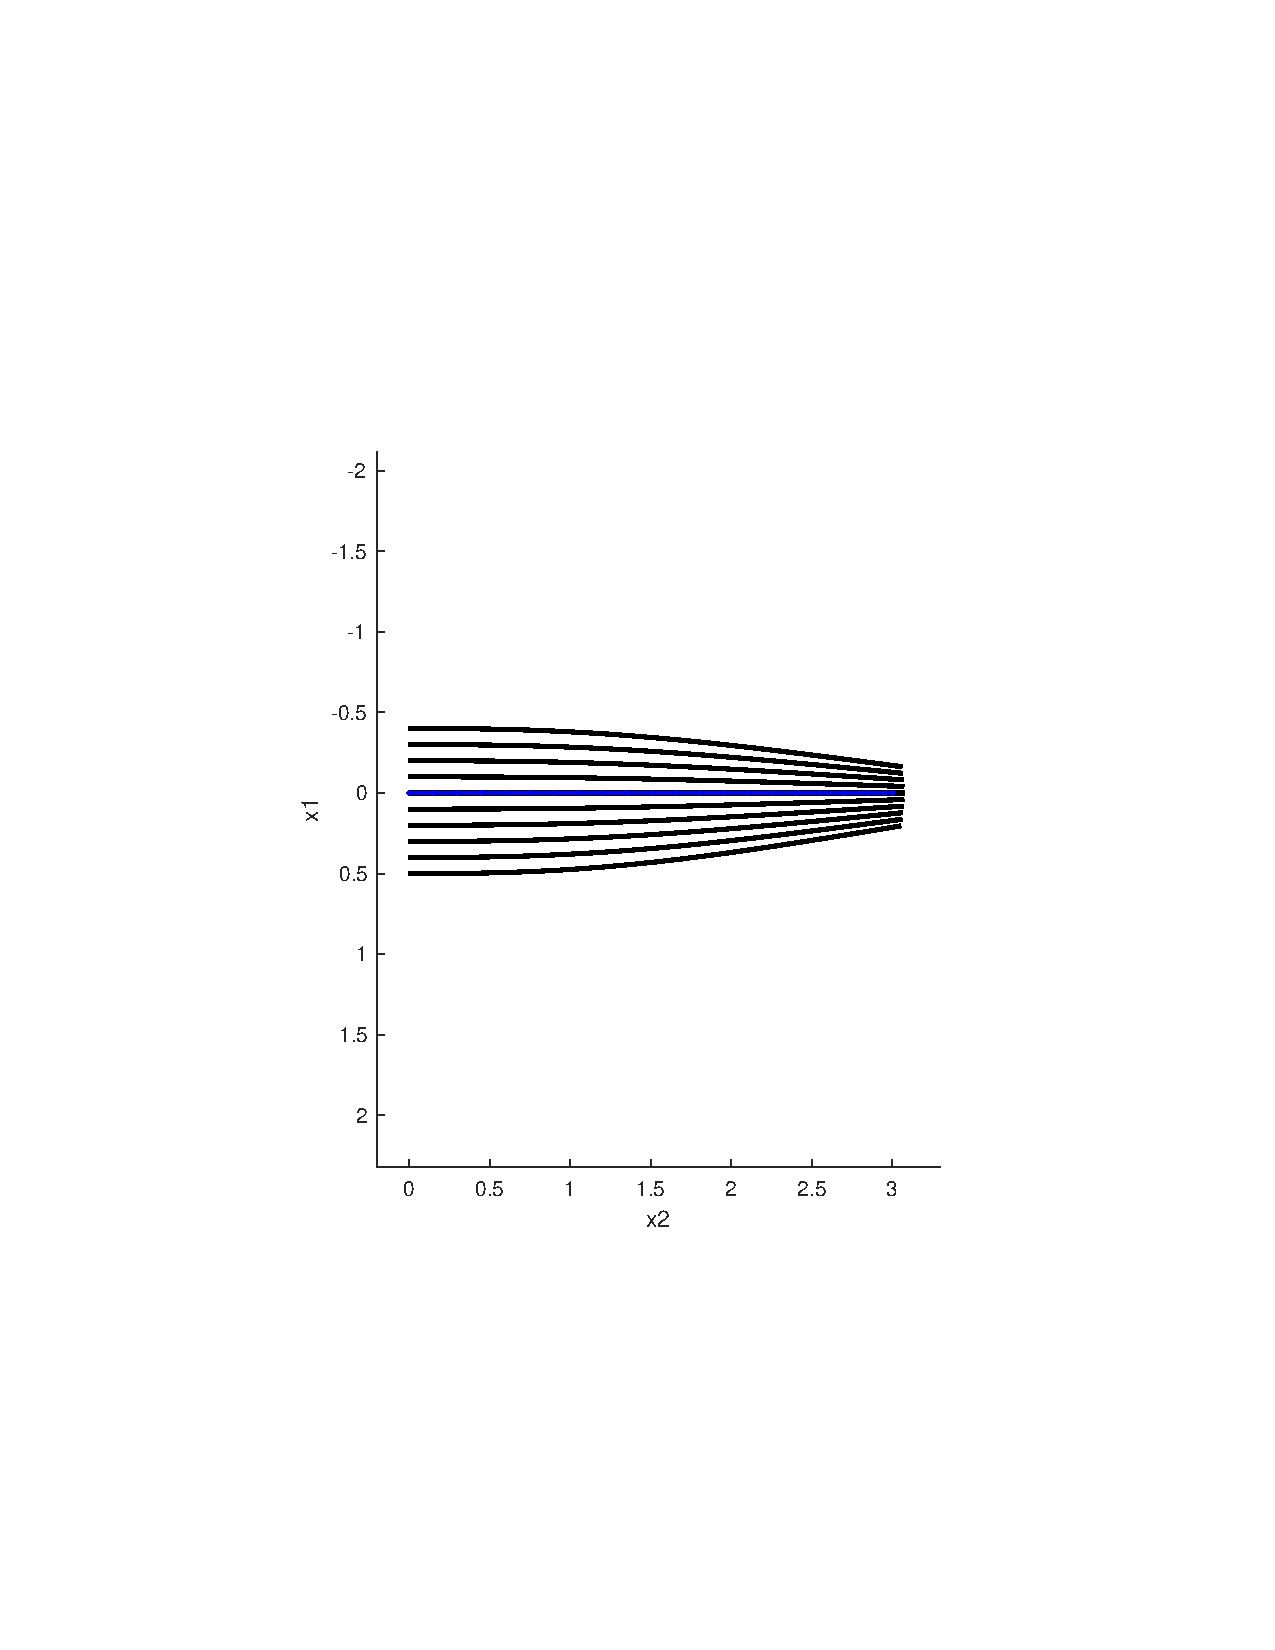
\includegraphics[scale=.5]{figures/preliminaries/montecarlofunnel}
  \caption{The simulation of N paths starting from a random point in the
    interval \(\sqb{-.5,.5}\), and controlled with a LQR controller.}
  \label{fig:monte-carlo-sim}
\end{figure}

\subsection{Funnels}
\label{sec:Funnels}

The term \funnel{} first appears in \cite{masonMechanicsManipulation1985}. The
\funnel{} definitions in this thesis is taken from a series of articles on
\funnel{}'s \cite{Tobenkin_2011} \cite{tedrakeLQRtreesFeedbackMotion2009,
  majumdarRobustOnlineMotion2013,
  majumdarFunnelLibrariesRealtime2017,ahmadi2014dsos}, with the main focus being
on \cite{majumdarFunnelLibrariesRealtime2017}. Here a \funnel{} is
mathematically defined as
\[
  \bar{\x}(0) \in \mathcal{X}_0 \implies \bar{\x}(t) \in F(t), \forall t \in
  \sqb{0,T}
\]
where \(\mathcal{X}_0\) is the set of initial conditions, \(\sqb{0,T}\) the time
interval, and \(F(t)\) is the set of states that the system can be in at time
\(t\).

\subsection{Defining funnels}

The funnel computations will be based on the \ac{SOS} theory developed
in~\cref{sec:Funnels}. Given a trajectory, the goal is to compute a robust
invariant set around the trajectory that will `guarantee' that the planner is
free from collisions during execution of the obtained motion plan. This robustly
invariant set is parameterized through Lyapunov function candidates, that, in
this case, will be based upon the \ac{PSD} matrix that the time-invariant
\ac{LQR} controller produces. The following presentations will be based
on~\cite{Tobenkin_2011, tedrakeLQRtreesFeedbackMotion2009,
  majumdarRobustOnlineMotion2013}, but mainly follow the formulations, and
syntax from~\cite{majumdarFunnelLibrariesRealtime2017}.

Thus, given the nonlinear dynamical system
\begin{equation}
  \label{eq:dynamicalsystem}
  \dot{\x} = f(\x(t), \uin(t))
\end{equation}
with \(\x(t)\) the state of the system at time \(t\) and \(\uin(t)\) the control
input. Assume that a open loop nominal trajectory \(\x_0 \colon [0,T]
\rightarrow \R^n\) with control input \(\uin_0 \colon [0,T] \rightarrow \R^n\) is
given, and define a change of coordinates into the error coordinate frame
\begin{align}
  \bar{\x}(t) &= (\x - \x_0)(t) \\
  \bar{\uin}(t) &= (\uin - \uin_0)(t).
\end{align}
Then, changing~\cref{eq:dynamicalsystem} to these new coordinates one obtains
\begin{equation}
  \label{eq:dynamicalsystem-coordinatechange}
  \dot{\bar{\x}} = \dot{\x} - \dot{\x}_0 = f(\x_0(t) + \bar{\x}(t), \uin_0(t) + \bar{\uin}(t)) - \dot{\x}_0(t)
\end{equation}

In order to compute a parameterized reachable set through \ac{SOS} programming
the system~\cref{eq:dynamicalsystem-coordinatechange} needs to be polynomial,
and parameterized by \(\x\) and \(t\), since the trajectory is parametrized by
\(\x\) and \(t\). Therefore, through the use of a \ac{TV-LQR} controller, the
control input can be eliminated from the dynamical equation, giving
\begin{equation}
  \label{eq:dynamicclosedloop}
  \dot{\bar{\x}} = f_{cl}(t,\bar{\x}(t)).
\end{equation}
However, the dynamical system may still not be polynomial, which is a necessary
condition in order for this to be verified using \ac{SOS} programming. Expanding
the system~\cref{eq:dynamicclosedloop} around the nominal trajectory \(\x_0\)
through a Taylor expansion of some degree high enough to capture the
nonlinearities of the system.

The goal is to parametrize a \textit{tight outer approximation} of the set of
states the system may transition into during the time interval \([0,T]\). Given
that \(F(t)\) is the set of states the system~\cref{eq:dynamicclosedloop} can be
in at time \(t\), then
\begin{equation}
  \label{eq:reachableset}
  \bar{\x}(0) \in \mathcal{X}_0 \implies \x(t) \in F(t), \, \forall t \in [0,T]
\end{equation}~\cite{majumdarFunnelLibrariesRealtime2017} 
where \(\mathcal{X}_0\) is the initial condition set, and \(F(t) \subset \R^n\)
is the finite time funnel for the system.

A funnel is defined in~\cite[Majumdar]{majumdarFunnelLibrariesRealtime2017} as
\begin{definition}
  \label{def:funnel}
  A funnel associatied with a closed-loop dynamical system \(\dot{\bar{\x}} =
  f_{cl}(t,\x(t))\) is a map \(F \colon [0,T] \rightarrow \mathcal{P}(\R^n)\),
  from the time interval \([0,T]\) to the power set (i.e., the set of subsets)
  of \(\R^n\) so that the sets \(F(t)\) satisfy the
  condition~\cref{eq:reachableset}.
\end{definition}
Thus, \(F(t)\) is the set of reachable states that the system can be in at time
\(t\).

Next, the reachable set is paramterized through the use of Lyapunov functions,
which yields
\begin{equation}
  F(t) = \set{\bar{\x}(t) \mid V(t, \bar{\x}(t) \leq \rho (t))}
\end{equation}
where \(\rho (t) \colon [0,T] \rightarrow \R^+\), is a function which limits the
size of the reachable set, and \(V(t,\bar{x}(t))\) is a Lyapunov function \(V
\colon [0,T] \times \R^n \rightarrow \R^+\).

Then, by setting \(\mathcal{X}_0 \subset F(0,\bar{\x})\), one can derive the
sufficient condition~\cref{eq:reachableset} for containing the reachable set in
the Lyapunov function paramterization
\begin{equation}
  \label{eq:funnelsufficient}
  V(t,\bar{\x}) = \rho(t) \implies \dot{V}(t,\bar{\x}) < \dot{\rho}(t), \, \forall t \in [0,T]
\end{equation}
with \(\dot{V}(t,\bar{\x})\) computed as
\begin{equation}
  \dot{V}(t,\bar{\x}) = \frac{\partial V(t,\bar{\x})}{\partial \x} f_{cl}(t,\bar{\x}) + \frac{\partial V(t,\bar{\x})}{\partial t}
\end{equation}

Currently there are no limitations on the functions \(V\) and \(\rho\), and
hence there exists infinitely many functions with different sized reachable sets
that satisfies~\cref{eq:funnelsufficient}, and is a valid funnel in the sense of
~\cref{def:funnel}. In order for efficient planning to take place, the motion
primitives, meaning the size of the funnels, should be as small as possible, and
it is therefore that the size of the funnels is minimized using the following
optimization problem~\cite{majumdarFunnelLibrariesRealtime2017}

\begin{align}
  \label{eq:funneloptimizationproblem}
  &\underset{V,\rho}{\text{inf}} \; &&\int_{0}^{T} \vol(F(t))\, dt \\
  &\text{subject to} && V(t,\bar{\x}) = \rho (t) \implies \dot{V}(t,\bar{\x}) < \rho (t) \, \forall t \in [0,T] \\
  && &\mathcal{X}_0 \subset F(0,\bar{\x}) \\
\end{align} 

\begin{figure}
  \centering
  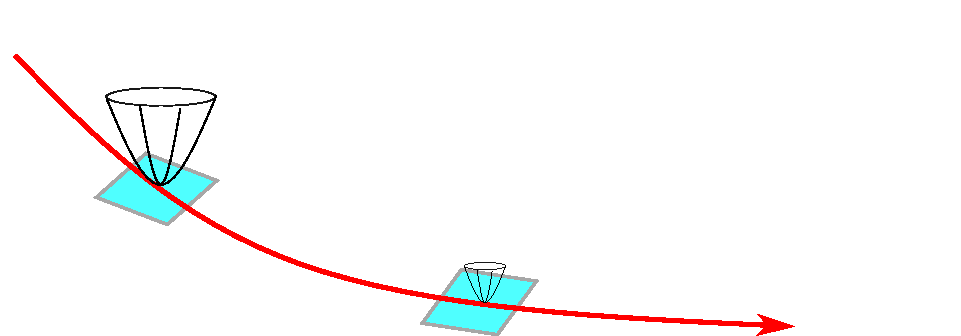
\includegraphics{figures/experiments/lyapunov_visualization}
  \caption{A visualization of the Lyapunov function along a trajectory, where
    the center of the Lyapunov function moves along the trajectory with time
    \(t\).}
\end{figure} 


\subsection{Formulating the optimization problem as a SOS program}

The optimization problem in~\cref{eq:funneloptimizationproblem} would prove
impossible to solve efficiently had it not been for recent advances in
mathematical convex numerical
optimization~\cite[Parillo]{parilloStructuredSemidefinitePrograms}, as in
general the problem involves searching over an infinite function space. While
the general optimization problem of searching through the infinite function
space is not amenable to efficient numerical computation, the problem can be
made computationally feasible through the use of a \ac{SOS} programming
approach.

Thus in order to make the problem amenable to a \ac{SOS} program, there are some
assumptions that need to be met by our problem formulation. Firstly the initial
condition set needs to be a \textit{semi-algebraic set}, (\ie{} parameterized by
polynomial inequalities),

\begin{equation}
  \mathcal{X}_0 = \set{\bar{\x} \in \R^n \mid g_{o,i}(\bar{\x}) \geq 0, \, i = 1,\ldots,N_0}
\end{equation}

Then rewriting~\cref{eq:funneloptimizationproblem}~as in terms of positivity and
equality constraints yields
\begin{equation}
  V(t,\bar{\x}) = \rho(t) \implies \dot{\rho}(t) - \dot{V}(t,\bar{\x}) > 0
\end{equation}
and
\begin{equation}
  g_{0,i}(\bar{\x}) \geq 0 \forall i \in \set{1,\ldots,N_0} \implies \rho(0) - V(0,\bar{\x}) \geq 0
\end{equation}
which, if these functions are both polynomial, is now in the form of a \ac{SOS}
optimization problem. Then through the use of the~\nameref{sec:s-procedure} one
arrives at the equations
\begin{align}
  &\dot{\rho}(t) - \dot{V}(t,\bar{\x}) - L(t,\bar{\x})\left[ V(t,\bar{\x}) - \rho(t) \right] - L_{t}(t,\bar{\x})\left[ t\left( T - t \right) \right]  && \text{is SOS}& \label{eq:sufficient-conditions}\\
  & \rho(0) - V(0,\bar{\x}) - \sum_{i}^{N_{0}} L_{0,i}(\bar{\x})g_{0,i}(\bar{\x}) && \text{is SOS}& \\
  & L_{t}(\bar{\x}), \, L_{0,i}(\bar{\x}) \; &&\text{are SOS}, \, \forall i \in \set{1,\ldots,N_{0}} \label{eq:sufficient-conditions3} \\
\end{align} 
where \(L\), \(L_{t}\), and \(L_{0,i}\) are multiplier
polynomials~\cref{sec:s-procedure}.

The goal is to make the parametrization of the reachable set as small as
possible, and therefore minimizing the cost
function~\cref{eq:funneloptimizationproblem}~. This is done
in~\cite{majumdarFunnelLibrariesRealtime2017}, through approximating the cost
function by first discretizing the problem and replacing the integral with a
finite sum
\begin{equation}
  \int_{0}^{T} \vol(F(t)) dt \rightarrow \sum_{k=1}^{N} \vol(F(t_{k})) \label{eq:discrete-costfunction}
\end{equation}
Since the Lyapunov function (\(V(t,\bar{x})\)) in this thesis is quadratic, it
can be written as
\begin{equation}
  V(t_{k}, \bar{\x}) = {\bar{\x}}^{T}S_{k}\bar{\x}, \, S_{k} \succeq 0
\end{equation}
which means that the set \(F(t_{k})\) is an ellipsoid in which the volume can be
minimized through maximizing the determinant of \(S_{k}\). Which in turn can be
transformed into a \ac{SDP} problem. If an upper bound on the cost
function~\cref{eq:discrete-costfunction} is introduced as
\begin{equation}
  \mathcal{E} (t_{k}) = \set{\bar{\x} \in \R^n \mid {\bar{\x}}^{T}S_{k}\bar{\x} \leq 1, \, S_{k} \succeq 0}
\end{equation}
where \( \mathcal{E} ( t_{k} ) \) is an ellipsoid containing the reachable set
\( F ( t_{k} ) \) at time \( t_{k} \). This containment constraint can be
equivalently expressed as
\begin{equation}
  V ( t_{k}, \bar{\x} ) \leq \rho(t_{k})  \implies {\bar{\x}}^{T}\matr{S}_{k}\bar{\x} \leq 1.
\end{equation}
Which when expressed using \ac{SOS} constraints
\begin{align}
  1 - {\bar{\x}}^{T}\matr{S}_{k}\bar{\x} - L_{\mathcal{E},k}(\bar{\x})\left[ \rho(t_{k}) - V(t_{k}, \bar{\x}) \right]  \qquad \text{is SOS}& \\
  L_{\mathcal{E},k}(\bar{\x}) \qquad \text{is SOS.}& \\
\end{align}

Then combining the cost function~\cref{eq:discrete-costfunction} with the
constraints~\cref{eq:sufficient-conditions,eq:sufficient-conditions3}, one
arrives at the optimization problem

{ % Mini environment scope
  \newcommand{\E}{\mathcal{E}} \renewcommand{\x}{\bar{x}}
  \begin{mini*}[1]
    { \substack { V, \rho, L, L_t,
        \\
        L_{0, i}, S_{k}, L_{\E, k} } } { \sum_{k = 1}^{N} \vol(\E(t_{k})) =
      \sum_{k = 1}^{N} \vol \p{\set{\x \mid \x^T \matr{S}_k \x \le 1}} } {} {}
    \addConstraint { \dot{\rho}(t) - \dot{V}(t,\x) - L(t,\x) \sqb*{ V(t,\x) -
        \rho(t) } - L_t (t,\x) \sqb*{t \p*{T - t}} }%
    {\text{ is SOS}} \addConstraint {\rho(0) - V(0, \x) - \sum_i^N L_{0, i}(\x)
      g_{0, i}(\x)}%
    {\text{ is SOS}} \addConstraint { 1 - \x^T \matr{S}_k \x - L_{\E, k}(\x)
      \sqb*{\rho(t_k) - V(t_k, \x)} }%
    {\text{ is SOS}} \addConstraint {S_k}%
    {\succeq 0}%
    {\quad \forall k \in \set{1, \ldots, N}} \addConstraint {L_t (t, \x),\,
      L_{0,i}(\x)}%
    {\text{ are SOS}}%
    {\quad \forall i \in \set{1, \ldots, N_0}} \addConstraint{}{}{\quad \forall
      k \in \set{1, \ldots, N}.}
  \end{mini*}
} % End optimization problem scope.

Which is the finite dimensional optimization problem needed in order to search
for a Lyapunov function candidate.

However, this optimization problem is not convex in general, as the first
constraints are \textit{bilinear} in the decision variables, since \(L\) and
\(V\) are multiplied together. However, the problem can be solved, although not
optimally, if \(V\) and \(\rho\) are held fixed, while the other decision
variables are free, the problem is possible to solve using \ac{SOS}
optimization. Likewise, fixing \(L\) and \(L_{\mathcal{E},k}\), creates another
\ac{SOS} optimization program. Therefore shifting between the two sets of
decision variables
\[
  \left( L,L_{t},L_{0,i},L_{\mathcal{E},k} \right)
\]
and
\[
  \left( V,\rho,L_{0,i},\matr{S}_{k} \right)
\]
\cite[Majumdar]{majumdarFunnelLibrariesRealtime2017} arrives at the following
algorithm for funnel computation

\begin{algorithm}[H]
  \caption{Funnel computation}
  \label{alg:funnelalgorithm}
  \DontPrintSemicolon \SetAlgoNoLine

  \KwIn{\(V\) and \(\rho\)} \KwOut{Funnel}

  \(cost_{prev} = \infty\)\; converged = false \; \While{\(!\; converged\)}{
    Optimization problem 1: \;
    \begin{align*}
      \underset{\substack{L,L_{t},L_{0,i},S_{k},L_{}}}{\inf}&  \sum_{k=1}^{N} \vol(\mathcal{E}(t_{k}))& \\    
      \text{subject to } & V \text{ and } \rho \text{ constant.}& \\
    \end{align*}\;
    Optimization problem 2: \;
    \begin{align*}
      \underset{\substack{V,\rho, L_{t},L_{0,i},S_{k}}}{\inf}&  \sum_{k=1}^{N} \vol(\mathcal{E}(t_{k}))& \\    
      \text{subject to } & L \text{ and } L_{\mathcal{E},k} \text{ constant.}& \\
    \end{align*}\;
    cost = \(\sum_{k=1}^{N} \vol(\mathcal{E}(t_{k}))\) \;
    \If{\(\frac{cost_{prev} - cost}{cost_{prev}} < \epsilon\)} {
      converged = true
    }\;
    \(cost_{prev} = cost\)\;
  }\;
\end{algorithm}

\subsection{Approximation via time-sampling}

It is often the case that the nomial trajectory \(x_{0} \colon [0,T] \rightarrow
\R^n\) is difficult to approximate with a low degree polynomial in
time~\cite{majumdarFunnelLibrariesRealtime2017}. As this can cause funnel
computation to take a lot of time, approximating the polynomial discretely
helps, but exactness will be lost, however the resulting funnels are shown to be
acceptable approximations, where exactness can be regained through increasing
the sampling rate~\cite{Tobenkin_2011}. If \(t_{k} \in [0,T]\), where \(k \in
\set{1,\ldots,N}\), the optimization equations become
\begin{mini}
  {\substack{V_{k}, \rho, L_{k},\\ L_{0,i}, S_{k},
      L_{\mathcal{E},k}}} % Optimization variables
  {\sum_{k=1}^{N}\vol(\mathcal{E}(t_{k})) = \sum_{k=1}^{N} \vol\left(
      \set{\bar{x} \mid {\bar{x}}^{T} S_{k} \bar{x} \leq 1}
    \right)} % Optimization function
  {\label{optidef:discrete}} % Label optimization problem
  {} % Optimization result
  % Constraints
  \addConstraint{\dot{\rho}(t_{k}) - \dot{V}_{k}(\bar{\x}) - L_{k}(\bar{\x})
    \left( V_{k}(\bar{\x}) - \rho(t_{k}) \right)} {\qquad} {\forall k \in
    \set{1,\ldots,N}} \addConstraint{\rho(t_{1}) - V_{1}(\bar{\x}) -
    \sum_{i}^{N_{0}} L_{0,i}g_{0,i}(\bar{\x})} {\, \text{is SOS}} {} %
  \addConstraint{1 - {\bar{\x}}^{T} S_{k} \bar{\x} - L_{\mathcal{E,k}} \left(
      \rho(t_{k}) - V_{k}(\bar{\x}) \right)} {\, \text{is SOS}\;} {\forall k \in
    \set{1,\ldots,N}} %
  \addConstraint{S_{k} \succeq 0} {} {\forall k \in \set{1,\ldots,N}} %
  \addConstraint{L_{0,i}(\bar{\x}), L_{\mathcal{E},k}} {\, \text{are SOS}} {\;
    \forall i \in \set{1,\ldots,N} \quad \forall k \in \set{1,\ldots,N}} %
\end{mini}

\subsection{Checking composability of Funnels}

In order for two \funnel's to be composable, the outlet of one \funnel{} needs
to be completely contained within the inlet of the other. This means that if
\(\mathcal{F}_1 = F_1(T)\) is the outlet of \funnel{} \(F_1\), and
\(\mathcal{F}_2 = F_2(0)\) is the inlet of \(F_2\), then
\begin{equation}
  \label{eq:funnel-subset}
  \mathcal{F}_1 \subseteq \mathcal{F}_2
\end{equation}
is required in order for the funnels to be composable. In this thesis this
composition checking is done off-line, prior to the running of the motion
planning stage of the \rrtfunnel{} algorithm. First however, it needs to verify
that the outlet of one \funnel{} is fully contained within the inlet of the
other.

In \cite[Majumdar and Tedrake, p.~47]{majumdarFunnelLibrariesRealtime2017}, two
funnels are sequentially composable if
\begin{definition}
  \label{def:funnel-composition}
  An ordered pair \((F1, F2)\) of funnels \(F_1 \colon [0,T_1] \rightarrow
  \mathcal{P}(\R^n)\) and \(F_2 \colon [0,T_2] \rightarrow \mathcal{P}(\R^n)\)
  is sequentially composable if \(F_1(T) \subseteq F_2(0)\).
\end{definition}

Thus
\[
  V_1(T_1,\bar{\x}) \leq \rho_1(T_1) \implies V_2(0,\bar{\x}) \leq \rho_2(0)
\]
is an equivalent condition to~\cref{eq:funnel-subset}, and which can be checked
through the following \ac{SOS} program.
\begin{align*}
  \text{Find } \; &L(\bar{x}) \\
  \text{s.t} \; &\rho_2(0) - V_2(0,\bar{\x}) - L(\bar{\x})
                  \left( \rho_1(T_1) - V_1(T_1,\bar{\x}) \right)
\end{align*}
\cite[Majumdar and Tedrake, p.~54]{majumdarFunnelLibrariesRealtime2017}

However in \cite[Majumdar and Tedrake]{majumdarFunnelLibrariesRealtime2017}, the
program is simply stated, and it can be helpful to take a look at the derivation
in order to gain a feel of the implementation of a \ac{SOS} program.

The \textit{S-procedure} enables us to limit our search to a semialgebraic set.
In this case, that set is \(\mathcal{F}_2 = \set{\x \in \R^n \mid
  V_2(0,\bar{\x}) \leq \rho_2(0)}\), any \(\x\) that is not in this set does not
concern us, which is why employing the \textit{S-procedure} is valid. In more
general terms this can be written
\[
  \x \in \mathcal{F}_2 \implies p(\x) \geq 0
\]
where \(p(\x)\) is the \ac{SOS} polynomial that is to be verified. In this case
\(p(\x)\) is \(V_2(0,\bar{\x})\). Thus in order to impose the implication define
\[
  q(\x) = V_2(0,\bar{\x}) - \rho_2(0) - L(\bar{\x}) \left( \rho_1(T_1) -
    V_1(T_1,\bar{\x}) \right)
\]
where \(q(\x)\) and \(L(\bar{\x})\) needs to be SOS polynomials.

\begin{example}

  As a simple example let's have a look at embedding a square within a circle.
  For good measure let's give the circle a radius of \(\sqrt{2}+\epsilon\), and
  the square a radius of \(1\), and center them both at the origin in the
  Euclidean plane.

  Starting with defining the set \(\beta\)
  \[
    \beta = \set{\x \in \R^2 \mid \norm{\x} \leq 2}
  \]
  using the manhattan metric. then the implication
  \[
    \x \in \beta \implies p(\x) \geq 0
  \]
  which can be formulated as
  \begin{align*}
    \beta &= \set{\x \in \R^2 \mid 1 \pm \x \geq 0 } \\
    p(\x) &= r^2 - x^2 - y^2
  \end{align*}
  where \(p(\x)\) is the parametrization of the circle, and \(\beta\) is the
  parametrization of the square with sides of length two. What needs to be shown
  is that \(p(x)\) is positive on the set \(\beta\). Through the
  \nameref{sec:s-procedure} this can be written as the search for a nonnegative
  polynomial \(L_{ineq,i}(\x)\) such that \(p(\x) \geq \left( L_{ineq,i}g
  \right)(\x)\). Thus
  \[
    q(\x) = p(\x) - \sum_{i=1}^{2}L_{ineq,i}(\x)g_{ineq,i}(\x)
  \]
  is required to be a \ac{SOS} polynomial, along with \(L_{ineq,i}\). From this
  it is seen that when a point satisfies \(g_{ineq,i}\) (\ie when \(\x \in
  \beta\)) the term \(\sum_{i=1}^{2}L_{ineq,i}(\x)g_{ineq,i}(\x)\) is negative,
  and hence \(p(x)\) must be nonnegative, which gives the desired implication.

  Solving this problem can be done using any of a number of \ac{SOS} modelling
  software. This example will rely on \cite[Yalmip]{Lofberg2004} and its
  \ac{SOS} programming functionality \cite{Lofberg2009} for \matlab.


  \lstinputlisting{figures/funnel/embededsquare.m}

  Which returns ``Composition succesful!'' for circles with radii larger than
  \(\sqrt{2}\) as expected.
\end{example}

\subsection{Cyclic coordinates and Lagrangian dynamics}
\label{subsec:cyclic-coordinates}

Given the Lagrangian \((\mathcal{L}(q_i, \dot{q_i}, t))\) of a dynamical system,
where the \((q_i)\) are the generalized coordinates of the system, and
\((\dot{q_i})\) are the generalized velocities. If the Lagrangian does not
contain the \((q_j)\) then \((q_j)\) is a cyclic coordinate of the system, and
the j-th Lagrangian has the form
\[
  \left( \frac{d}{dt} \right) \left( \frac{\partial \mathcal{L}}{\partial
      \dot{q_j}} \right) = \mathrm{const}
\]
This means that any \((q_j)\) fullfilling the above criteria can be freely moved
around in the state-space, yet yield the same dynamical solution of the system.


